\documentclass[12pt,a4paper]{scrartcl}

\usepackage[english]{babel}
\usepackage[T1]{fontenc}
\usepackage{graphicx, subfig}
\usepackage[document]{ragged2e}
\usepackage{lmodern}
\usepackage{color}
\usepackage{amsmath}
\usepackage{graphicx}
\usepackage{amsmath}
\usepackage{amsfonts}
\usepackage{amssymb}

% Für Verwendugn von Utnerstrichen ohne Escaping
\usepackage{underscore}

% Für Referenzen mit eigenem Text
\usepackage{hyperref}

% Für Codeblöcke
\usepackage{listings}

% Für Verwendung von Farben
\usepackage[usenames,dvipsnames,svgnames,table]{xcolor}

% Für Vektor-Pfeile
\usepackage{esvect}

% Für Größe der Seitenränder
\usepackage[margin=1in,footskip=0.5in]{geometry}

% Für Tabellen über Seiten hinweg
\usepackage{longtable}

% Für Header and Footer
\usepackage[automark]{scrpage2}

% Für Bildunterschriften
\usepackage[aboveskip=2pt, belowskip=10pt]{caption}

% Für Quellenverzeichnis
\usepackage[style=authoryear]{biblatex}
\addbibresource{\jobname.bib}

% Für animierte Grafiken
\usepackage{animate}

% Formatierung für Hyperref-Referenzen
\hypersetup{
	colorlinks,
	linkcolor={blue!50!black},
	citecolor={blue!50!black},
	urlcolor={blue!80!black}
}

% Generelle Formatierung für Code-Blöcke
\lstset{ %
	columns=fullflexible,
	keepspaces=true,
	frame=single,
	breaklines=true,
	breakautoindent=true,
	gobble=0,
	tabsize=2,
	belowskip=0pt
}

% Formatierung für Pseudo-Code
\lstdefinelanguage{PSEUDO} 
{ 
	xleftmargin=0pt, 
	xrightmargin=0pt,
	basicstyle=\small\ttfamily\color{Black},
	morekeywords={for, each, if, else},	
	keywordstyle = {\color{Orange}},
	sensitive=false,
	morecomment=[l]{//},
	morecomment=[s]{/*}{*/},
	morestring=[b]"
}

\newcommand{\mybox}{%
    \collectbox{%
        \setlength{\fboxsep}{1pt}%
        \fbox{\BOXCONTENT}%
    }%
}

\makeatother
\title{Wave simulation in OpenGL}
\author{Fabian Niehaus, Tuyet Nguyen}
\date{Juni 22, 2018}

\makeatletter

%% Generelle Kopf- und Fußzeilendefinition
\pagestyle{scrheadings}
%\automark[section]{subsection} 
\clearscrheadfoot
\ihead[]{\@title}
%\ohead[]{\rightmark}
\ifoot[]{\@author}

\begin{document}

\begin{titlepage}
	\centering
	\ \\[2cm]
	{\huge\textbf{\@title}} 
	\\[3cm]
	\large
	\textbf{Field of study:} Media informatics \\
	\textbf{Semester:} 4
	\\[2cm]
	\textbf{Date}: \@date
	\\[2cm]
	\textbf {Authors:}
	\\Fabian Niehaus
	\\Tuyet Nguyen
\end{titlepage}

\newpage
%% Seitezahl auf 0 setzen
\setcounter{page}{0}
\tableofcontents
\newpage
\listoffigures

\newpage
%% Seitennummern einblenden
\ofoot[]{\pagemark}
\normalsize

\section{Abstract}
In this project we will build a C++ application to simulate circular waves on a 3D mesh surface. We will also simulate reflection using the Image Source Method. We will use QT Creator for programming, QT for window management and OpenGL for 3D rendering.



\section{Wave theory}\label{wave-theory}

\begin{center}
	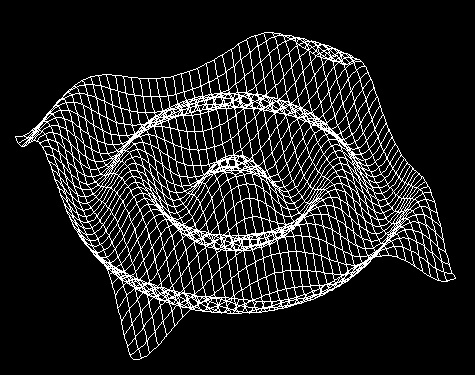
\includegraphics[width=0.5\textwidth]{Images/Concept.jpg}
	\captionof{figure}{Circular sine wave (\citefield{waveConceptPic}{title} \citefield{waveConceptPic}{year})}
\end{center} 

In this project, we will use a basic cosine wave with variable parameters for amplitude, wavelength and point of origin (POI). This function is derived from a complex wave function of which we only use the real part.
\begin{lstlisting}[language=PSEUDO]
X = linspace( -50, 50, 201); % 201 samples from -50 to 50

% complex wave centered at x=-17, wave length = 8.5
F = exp( i*abs(X*2*pi/8.5)); % first wave
freq = 10;
for t=0:.001:1 % one second in steps of milliseconds
	phi = -2*pi*freq*t; % phase shift due to time delay
	F1 = exp( i* phi) * F; % add phase shift to F
	plot( X, real(F1)); % plot real part
	axis([-50 50 -5 5]); % define figure scale
	drawnow
end
\end{lstlisting}
\captionof{figure}{Complex Wave Equation in Matlab \parencite{cgLec}} 

A cosine wave with circular expansion can be calculated using the formula
$$P(x,z,t) = a * \cos(k * {\Delta} + \Phi) $$
\captionof{figure}{Circular cosine wave function}
\ \\
where \textit{a} describes the wave's amplitude, \textit{k} describes the wave number, ${\Delta}$ describes the distance to the wave's OP and $\Phi$ describes the phase shift.\\
\ \\
\begin{center}
	\begin{tabular}{ll}
		Wavelength: & $l$ \\
		Time: & $t$ \\
		Wave Number: & $k = \frac{2\pi}{l}$ \\
		Phase Shift: & $\Phi = -2 * \pi * f * t$ \\
		Frequency: & $f = \frac{c}{l}$ \\
		Phase Velocity: & $c = g * l * 2\pi$ \\
		Gravitational Acceleration: & $g = 9.81 m/s^2$
	\end{tabular}
	\captionof{figure}{Variable definitions \parencite{waterSim}}
\end{center}
\ \\
As this project aims for a somewhat realistic behaviour of the wave, the amplitude needs to diminish with increasing distance to the wave's point of origin. In order to accomplish this effect, the distance to OP is factored in a second time:

$$P(x,z,t) = a * \cos(k * {\Delta} + \Phi) * \frac{1}{{\Delta}+1} $$
\captionof{figure}{Circular cosine wave function with diminishing amplitude}
\ \\
As ${\Delta}$ equals $0$ at the wave's OP and multiplier needs to always be less than $1$, $1$ is added to ${\Delta}$ in the multiplier's divisor.\\
\ \\
Using this formula, the height for every point of a mesh can be calculated. This formula can also be used to calculate multiple overlapping waves. In that case, the new height for a point is the sum of all waves.\\

\section{Realisation}

\subsection{Creating a basic interface with QT}
First off, we create a new QT widget application. This allows us to use QT Creators design feature to set up our application's interface. A new QOpenGLWidget is placed and will be used as a placeholder for a new custom class inheriting QOpenGLWidgets functionality. This class, called OGLWidget, needs to implement the following methods: initializeGL (for setting up OpenGL), paintGL (for doing the actual rendering), resizeGL (for handling resizes of the display window). Additionally, the functions stepAnimation SetMaterialColor and InitLightingAndProjection\footnote{Taken from Prof. Dr. Martin Hering-Bertrams OpenGL_Example} are used.

\subsection{Creating the data structure}
The data structure is separated in different classes. \\
The class "Wave" contains a single wave's parameters such as wavelength \textit{l}, amplitude \textit{a} and point of origin $\Delta$. It also holds the values for wave number \textit{k}, phase speed \textit{c} and frequency \textit{f}, which are calculated when the object is instanciated. \\ 
The class "Wavesurface" contains the surface mesh as well as the logic for calculating the mesh height.

\subsection{Creating the surface mesh}
The surface mesh consists of a two dimensional list of QVector3Ds, QT's own implementation of a three value vector. These vectors store a single point's x, y and z coordinates. We settled on a dimension of 50 x 50, which is sufficient from both a graphical and a performance point of view.\\
The mesh is located in the x-z-plane, meaning the waves' 'height' is calculated in y-direction.\\

\subsection{Calculating the mesh height}
Using the formula $P(x,z,t) = a * \cos(k * {\Delta} + \Phi) * \frac{1}{{\Delta}+1} $ explained under \hyperref[wave-theory]{Wave Theory}, a function  which calculates the sum of amplitudes for all waves for every point of the mesh is implemented.

\begin{lstlisting}[language=PSEUDO]
for each mesh row
	for each mesh column
		double height //Hoehe
		for each wave
			add result of formula stated above to height
		set y of current Point to height
\end{lstlisting}
\captionof{figure}{Calculating mesh height (pseudo code)} 

\subsection{Rendering}
In order to display the mesh on the screen, OpenGL needs to be instructed to render the points. Before rendering, the original coordinate system is rotated by 45° in positive x and negative y direction so the mesh is visible from an angle. Then, the specific rendering methods are called.

\subsubsection{Rendering as a wireframe}
First, the mesh is draw as a wireframe using the method drawMeshWireFrame(). This function connects all mesh points into triangles and the draws them on the screen.

\begin{center}
	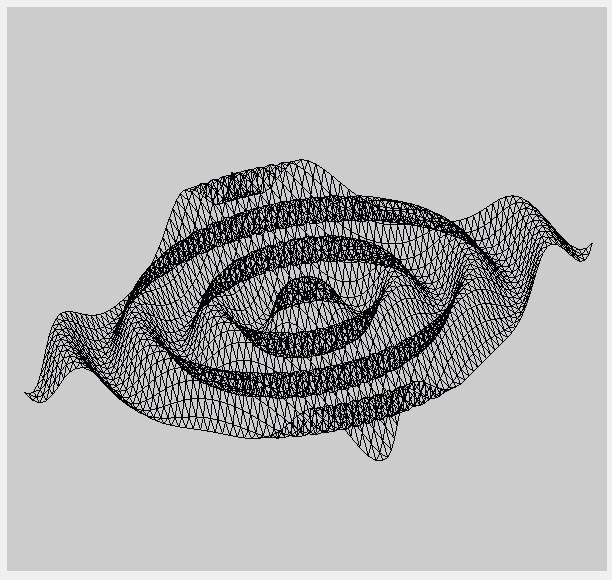
\includegraphics[width=0.5\textwidth]{Images/RenderingWireframe.jpg}
	\captionof{figure}{Rendering as wireframe}
\end{center} 

\subsubsection{Rendering as an opaque surface}
After drawing the object as a wireframe we want to draw it as an opaque surface with lighting. This is being achieved in the method drawMeshQuads() which connects all points into quads. This time using GL_Quads, the four vertices of a quad are connected and the area inbetween is filled. The normal vector for this is calculated using the cross product of the two diagonals vectors.

\begin{center}
	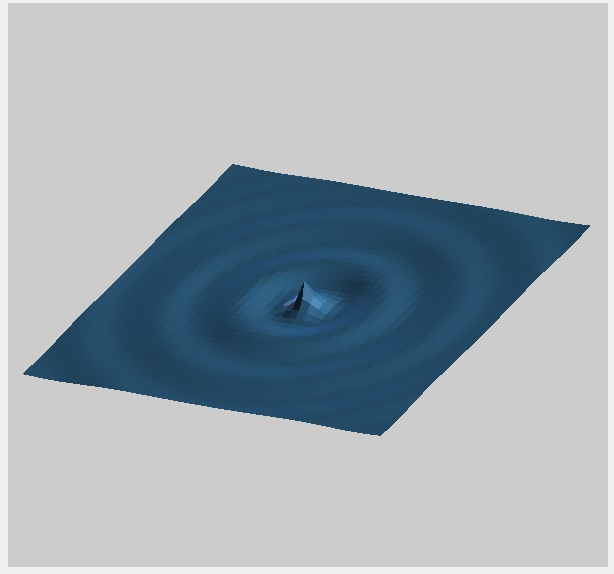
\includegraphics[width=0.5\textwidth]{Images/RenderingOpaque.jpg}
	\captionof{figure}{Rendering as opaque surface}
\end{center} 

\subsection{Wave peflection}
In this project, we also aimed to simulated reflection of the waves as if our mesh was a body of water located inside a rectangular container.

\begin{center}
	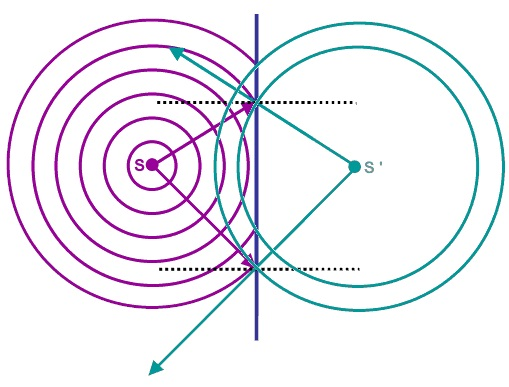
\includegraphics[width=0.5\textwidth]{Images/Reflection.jpg}
	\captionof{figure}{Circular Waves reflecting on a straight barrier \parencite{reflectionConceptPic}}
\end{center}

In order to achieve this effect, the so called Image Source Method was used. This method simulates reflection by placing another wave on the other side of the felection obstacle. The OP of this additional wave is placed at the same distance to the obstacle that the original wave's OP is at.

\begin{center}
	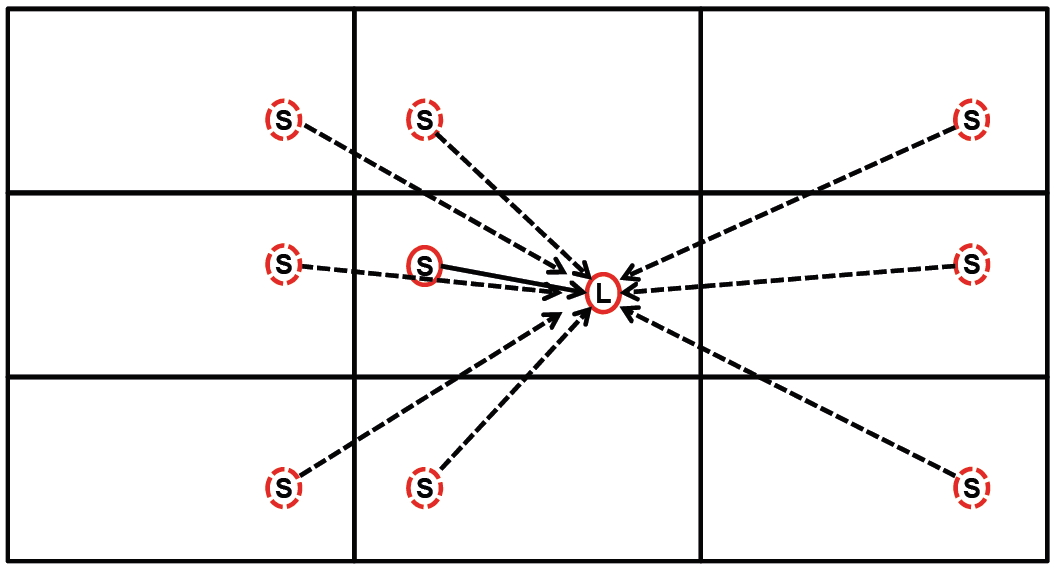
\includegraphics[width=0.6\textwidth]{Images/ImageSourceMethod.jpg}
	\captionof{figure}{Image Source Method \parencite{imageSourcePic}}
\end{center}

To ensure an acceptable level of reflection, we placed an additional wave in each of the eight neighboring tiles. This way, the original wave is reflected from each direction.

\begin{lstlisting}[language=PSEUDO]
meshX = dimension of mesh in x direction
meshZ = dimenstion of mesh in z direction
origX = x value of original wave's OP
origX = z value of original wave's OP

w1_Origin = (-1 * meshX - origX, mesh/ - origZ); // links oben
w2_Origin = (origX, mesh/ - origZ); // oben
w3_Origin = (meshX - origX, mesh/ - origZ); // rechts oben
w4_Origin = (-1 * meshX - origX, origZ); // links
w5_Origin = (meshX - origX, origZ); // rechts
w6_Origin = (-1 * meshX - origX, -1 * mesh/ - origZ); // links unten
w7_Origin = (origX, -1 * mesh/ - origZ); // unten
w8_Origin = (meshX - origX, -1 * mesh/ - origZ); // rechts unten
\end{lstlisting}
\captionof{figure}{Calculating OPs for reflection waves (pseudo code)}

\subsection{Dynamic parameters}
In the last step, user inputs for dynamic parameters were implemented. The following wave and program parameters can be set at runtime:
\begin{itemize}
	\item Amplitude
	\item Wavelength
	\item Point of origin
	\item Reflection (On / Off)
\end{itemize}

Inputs are made via sliders for numerical values and a checkbox for on/off values.
\begin{center}
	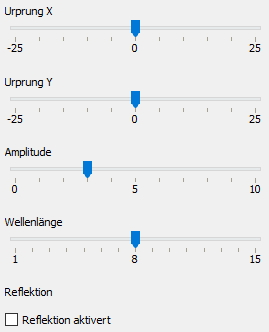
\includegraphics[width=0.5\textwidth]{Images/Inputs.jpg}
	\captionof{figure}{User Inputs}
\end{center}

Every slider is connected to a corresponding function with the program using QT's SIGNAL-SLOT mechanism (compare to \citefield{slidersExample}{title}, The QT Company \citefield{slidersExample}{year}). For example, the slider for the OPs x coordinate is connected to the updateWaveX() method of the program.\\
Whenever an input is changed, the updateWaves() function is called from the connected funtion. Every value except the changed one is copied from the current state and all waves are subsequently deleted and then newly created with the new parameter.

\begin{lstlisting}[language=PSEUDO]
delete all waves
create new origin wave (amplitude, wavelength, OP)
if relfection is active
	create the 8 corresponding reflection waves
\end{lstlisting}
\captionof{figure}{Updating the waves (pseudo code)}

\subsection{Finished application}
The following application is the functional result of implementing all aspects listed above:

\begin{center}
	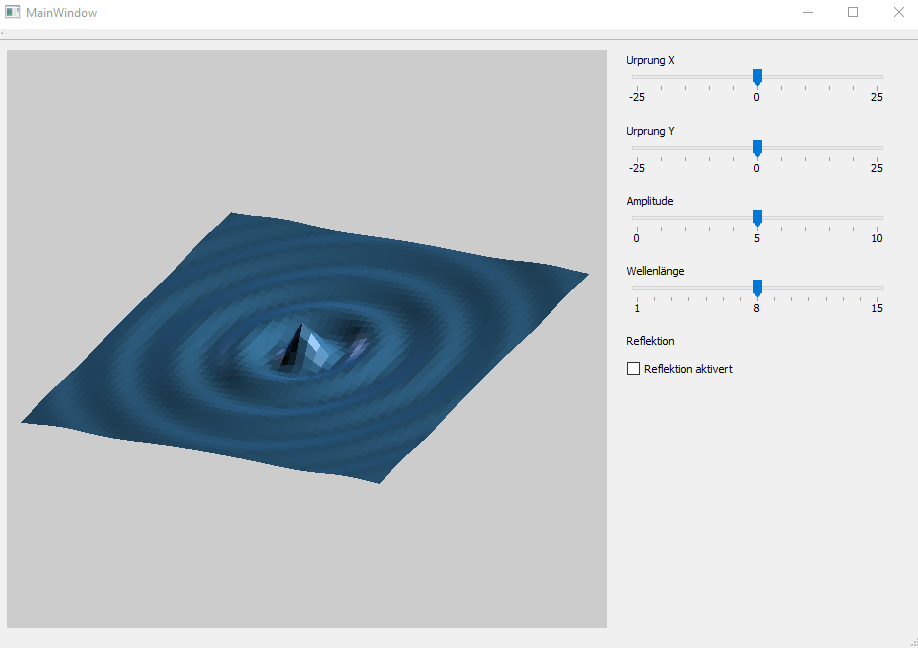
\includegraphics[width=0.9\textwidth]{Images/FinalProduct/FinalProduct0.png}
	\captionof{figure}{Finished application (1)}
\end{center}
\begin{center}
	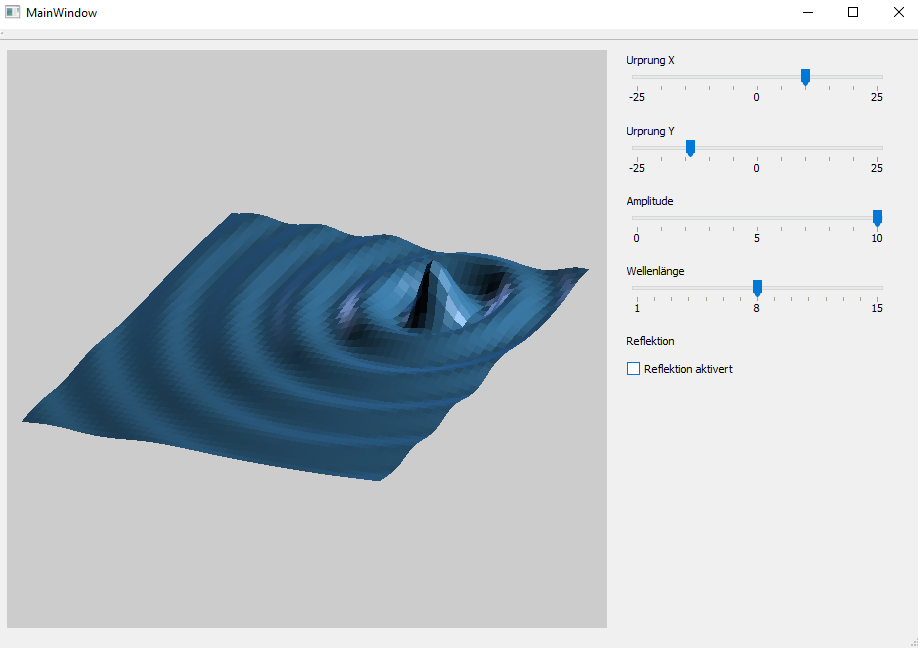
\includegraphics[width=0.9\textwidth]{Images/FinalProduct/FinalProduct234.png}
	\captionof{figure}{Finished application (2)}
\end{center}
\begin{center}
	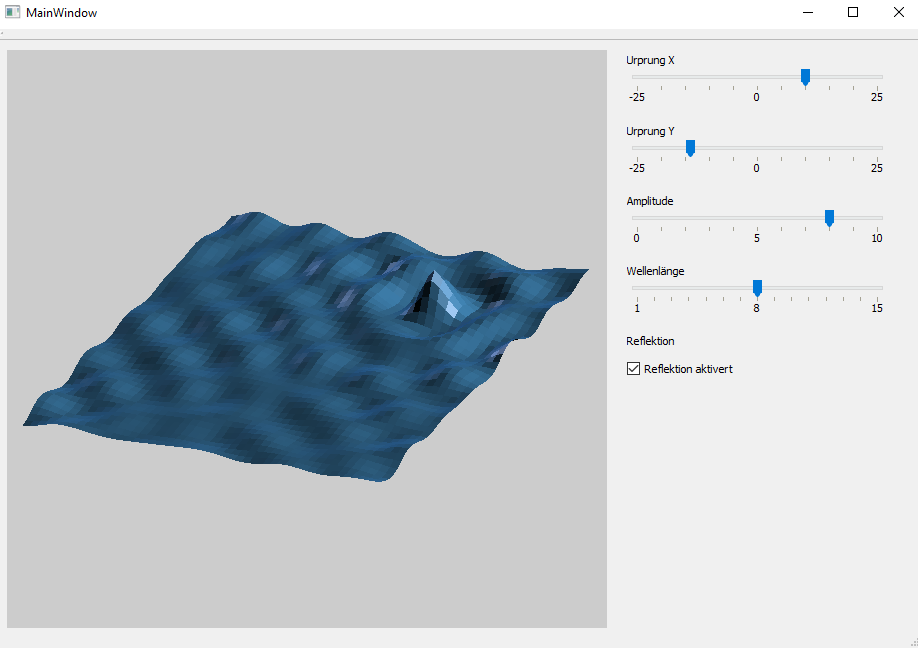
\includegraphics[width=0.9\textwidth]{Images/FinalProduct/FinalProduct306.png}
	\captionof{figure}{Finished application (3)}
\end{center}

\section{Conclusion}
We were able to create a simple wave simulator with wave reflection and user inputs. We gained deeper understandig of the mathematics involved in wave calculation and reflection.\\
Further improvements to the simulation could be made by using so-called Gerstner waves instead of cosine wave. These waves resemble the actual behaviour of water more closely. The mesh calculations could also be offloaded into the GPU via the use of shaders. Shadres would also allow for more realistic display of water, including refraction and skybox reflection.\\

\section{Acknowledgements}
\begin{itemize}
	\item The Wolfram Alpha computational engine for helping out with some of the mathematics involved
	\item The QT Company, GitHub, the developers of OpenGL, the developers of TeXStudio and the developers of MiKTEX for letting us use their software free of charge
	\item Prof. Dr. Martin Hering-Bertram for providing the OpenGL example code for coloring, lighting and projection used in the project
\end{itemize}

\section{References}

\printbibliography[title=Sources,nottype=misc]
\printbibliography[title=Pictures,type=misc]

\end{document}